\documentclass[nobib]{tufte-handout}

\title{Lecture 10: Connectivity $\cdot$ 1MA020}

\author[Vilhelm Agdur]{Vilhelm Agdur\thanks{\href{mailto:vilhelm.agdur@math.uu.se}{\nolinkurl{vilhelm.agdur@math.uu.se}}}}

\date{20 November 2023}


%\geometry{showframe} % display margins for debugging page layout

\usepackage{graphicx} % allow embedded images
  \setkeys{Gin}{width=\linewidth,totalheight=\textheight,keepaspectratio}
  \graphicspath{{graphics/}} % set of paths to search for images
\usepackage{amsmath}  % extended mathematics
\usepackage{booktabs} % book-quality tables
\usepackage{units}    % non-stacked fractions and better unit spacing
\usepackage{multicol} % multiple column layout facilities
\usepackage{lipsum}   % filler text
\usepackage{fancyvrb} % extended verbatim environments
  \fvset{fontsize=\normalsize}% default font size for fancy-verbatim environments

\usepackage{color,soul} % Highlights for text

% Standardize command font styles and environments
\newcommand{\doccmd}[1]{\texttt{\textbackslash#1}}% command name -- adds backslash automatically
\newcommand{\docopt}[1]{\ensuremath{\langle}\textrm{\textit{#1}}\ensuremath{\rangle}}% optional command argument
\newcommand{\docarg}[1]{\textrm{\textit{#1}}}% (required) command argument
\newcommand{\docenv}[1]{\textsf{#1}}% environment name
\newcommand{\docpkg}[1]{\texttt{#1}}% package name
\newcommand{\doccls}[1]{\texttt{#1}}% document class name
\newcommand{\docclsopt}[1]{\texttt{#1}}% document class option name
\newenvironment{docspec}{\begin{quote}\noindent}{\end{quote}}% command specification environment

\include{mathcommands.extratex}

\begin{document}

\maketitle% this prints the handout title, author, and date

\begin{abstract}
\noindent
We study the notion of the \emph{connectivity} of a graph, which quantifies \emph{how} connected a graph is. Then we prove some structure theorems about $2$- and $3$-connected graphs.
\end{abstract}

We already began our study of connectivity in the exercise session, but let us restate the central definitions again.

\begin{definition}
  A simple graph $G = (V,E)$ is called \emph{$k$-connected} if $\abs{V} > k$ and $G[V\setminus X]$ is connected for every $X \subseteq V$ with $\abs{X} < k$. The \emph{connectivity} of $G$ is the largest $k$ for which $G$ is $k$-connected, denoted $\kappa(G)$.\sidenote[][]{For infinite graphs this might, of course, not be well defined, since there might be no \emph{largest} such $k$.
  
  \begin{xca}
    Give an example of a graph which is $k$-connected for \emph{every} $k$.
  \end{xca}} 
\end{definition}

\begin{figure}
  \centering
  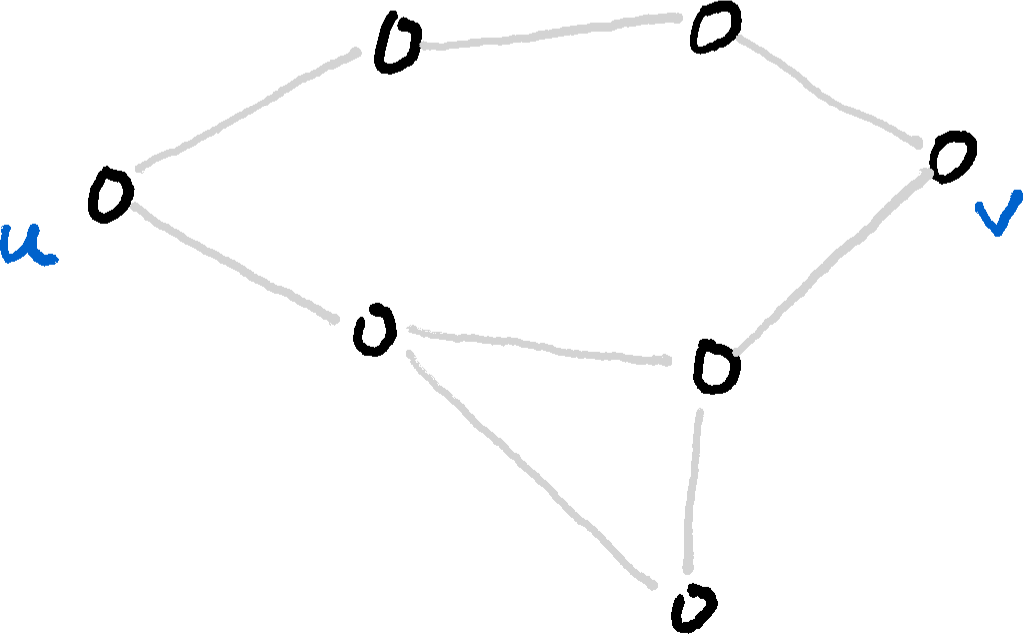
\includegraphics[width=0.6\textwidth]{graphics/L10_connectivity/twoconnected_graph.png}
  \caption[][1.5cm]{A graph of connectivity two. Removing any single vertex does not disconnect the graph, but there are obviously ways to remove two vertices to disconnect it.}
  \label{fig:twoconnected_graph}
\end{figure}

\begin{example}
  Every graph is zero-connected,\sidenote[][]{Unless you consider the ``empty graph'' $(\emptyset, \emptyset)$ to be a graph.} and every connected graph on at least two vertices is one-connected. $K_n$ is $n-1$-connected, as is a complete graph with one edge removed, and $K_{a,b}$ is $\min(a,b)$-connected. The graphs of connectivity zero are precisely the disconnected graphs and $K_1$.
\end{example}

\begin{definition}
  Let $G = (V,E)$ be a graph, and let $v, w \in V$ be two vertices and $A, B \subseteq V$ two sets of vertices.

  A set $X \subseteq V$ \emph{separates} $v$ from $w$ if $X \not\ni v, w$ and every path from $v$ to $w$ contains at least one vertex from $X$. We denote the minimum size of a set separating $v$ from $w$ by $\kappa(v,w)$.

  A set $X \subseteq V$ \emph{separates} $A$ from $B$ if every path from a vertex in $A$ to a vertex in $B$ contains at least one vertex of $X$. Notice that here we do not require $A$, $B$, and $X$ to be disjoint -- and in fact if $A\cap B\neq \emptyset$ we must have this intersection contained in $X$, or the lazy path starting and ending at the same vertex in $A\cap B$ would prevent separation.
\end{definition}

\begin{lemma}\label{lemma:connectivity_is_min_of_pairwise_connectivity}
  For a graph $G = (V,E)$ that is not a complete graph, we have
  $$\kappa(G) = \min_{\substack{u, v \in V\\u\sim v \not\in E}} \kappa(u,v).$$

  \begin{proof}
    Since $G$ is not complete, $\kappa(G)$ equals the minimum size of a set $X \subseteq V$ whose removal disconnects the graph.\sidenote[][]{Since it is not complete, there exists a pair of vertices without an edge between them. Removing all vertices but these two definitely disconnects the graph.} Let $X$ be a minimal such set, and so since $G[V \setminus X]$ is disconnected we can find $x_0$ and $y_0$ from different components, which are thus separated by $X$. So $\min_{x,y \in V} \kappa(x,y) \leq \abs{X} = \kappa(G)$.

    Conversely, let $x_0$ and $y_0$ be two non-adjacent vertices such that $\kappa(x_0, y_0)$ attains this minimum. Then there exists a separating set $X$ for $x_0$ and $y_0$ of size $\kappa(x_0, y_0) = \min_{x,y \in V: x\sim y \not\in E} \kappa(x, y)$. So in particular a set of this size suffices to disconnect $G$, and hence $\kappa(G) \leq \min_{x,y \in V: x\sim y \not\in E} \kappa(x, y)$.
  \end{proof}
\end{lemma}

We are now ready to show Menger's theorem, the content of which is that we could also have defined connectivity in terms of independent paths.

\begin{theorem}[Menger]
  Let $G$ be a graph, and let $u$ and $v$ be two non-adjacent vertices of $G$. Then $\kappa(u,v)$, the minimum size of a set that separates $u$ and $v$, equals the maximum size of a set of independent paths from $v$ to $w$, where we say that two paths are independent if they share only their start and end point.

  \begin{proof}
    We will again use a clever flow network construction to prove this with the max-flow min-cut theorem.\sidenote[][]{So when I said in an earlier lecture that we were done applying this technique, I was obviously wrong.} The way we construct our flow network is to first replace every edge $x\sim y$ by two edges $x\to y$ and $y\to x$. Then, for every vertex $x$, except $u$ and $v$, we split it into two vertices $x_i$ and $x_o$, and replace every edge incoming to $x$ with one to $x_i$, and likewise every edge going out of $x$ with one going out of $x_o$. Finally, we add an edge from $x_i$ to $x_o$.

    \begin{figure}
      \centering
      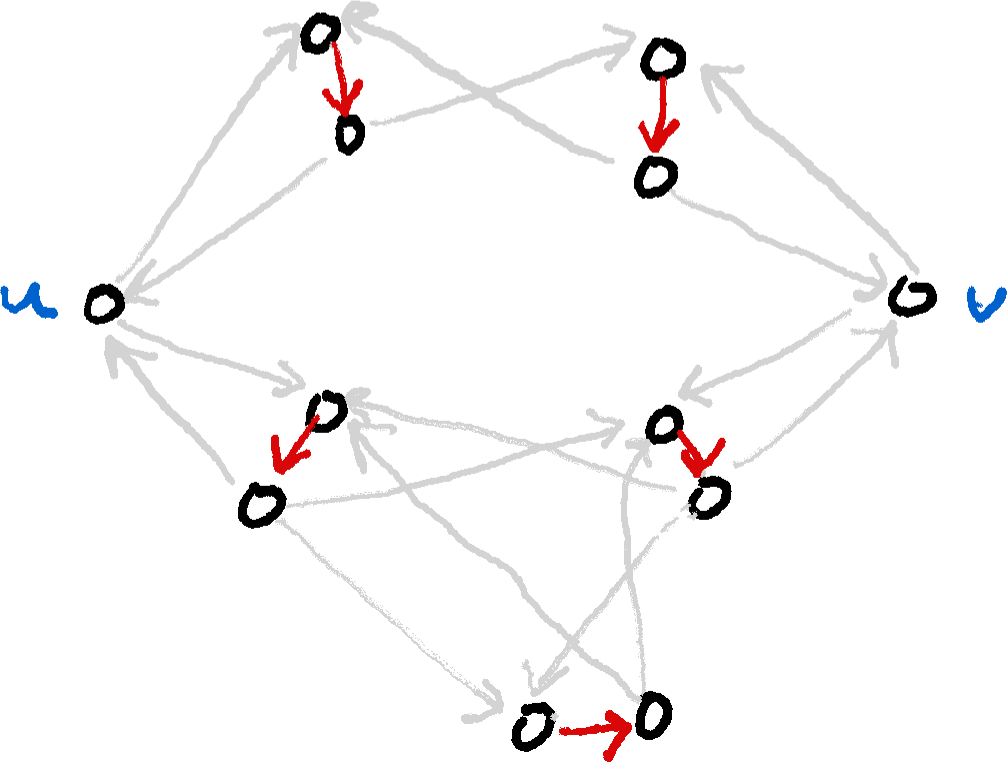
\includegraphics[width=0.6\textwidth]{graphics/L10_connectivity/menger_theorem_construction.png}
      \caption[][1.5cm]{The result of applying our flow network construction to the graph in Figure \ref{fig:twoconnected_graph}. Red edges have capacity one, grey edges have infinite capacity.}
      \label{fig:menger_thm_construction}
    \end{figure}

    We declare all edges to have infinite capacity, except for the ones from $x_i$ to $x_o$, which have capacity $1$.

    It is clear that an integer flow in this graph corresponds precisely to a set of independent paths from $u$ to $v$, since our construction with an edge of capacity one for each vertex means each vertex can only be used zero or one times. So a maximum flow corresponds to a maximum set of independent paths.

    Likewise, it is easy to see that a cut must, to have finite capacity, cut only through the edges of weight one, which correspond to vertices in the original graph, and their capacity is precisely the number of such vertices it cuts. So the capacity of a minimum cut is the minimum size of a set of vertices separating $u$ from $v$.

    So, by the max-flow min-cut theorem, the maximum number of independent paths equals the minimum size of a separating set.
  \end{proof}
\end{theorem}

At first glance, the following corollary looks like it should be entirely trivial, but it actually requires a little bit of work.

\begin{theorem}[Menger, global version]
  A graph is $k$-connected if and only if it contains $k$ independent paths between any two vertices.

  \begin{proof}
    Let $G = (V,E)$ be a graph. If $G$ has $k$ or fewer vertices, it is by definition not $k$-connected, and it is clearly impossible for there to be $k$ independent paths at all, since there are just too few vertices. Similarly, if $G$ is complete on more than $k$ vertices, we see easily that it is both $k$-connected and has the requisite number of independent paths. So we lose no generality in assuming $G$ is a non-complete graph on more than $k$ vertices.

    If $G$ is $k$-connected, then $\kappa(G) \geq k$ and hence $\kappa(u,v) \geq k$ for any two non-adjacent vertices $u$ and $v$ by Lemma \ref{lemma:connectivity_is_min_of_pairwise_connectivity}. By Menger's theorem, $u$ and $v$ are thus connected by at least $k$ independent paths.

    What remains to be shown is that we also have enough independent paths in the case where $u$ and $v$ \emph{are} adjacent. So assume for contradiction that there are at most $k-1$ independent paths from $u$ to $v$. After removing the edge $u \sim v$ from $G$ to get a graph $G'$, we are left with at most $k - 2$ independent paths from $u$ to $v$ in $G'$.

    Hence, by Menger's theorem, we can separate $u$ from $v$ by a set $X$ of size at most $k-2$ in $G'$. Since $G$ has more than $k$ vertices, there must be a vertex $w \in V \setminus (X \cup \{v,w\})$. Then this $w$ is separated by $X$ in $G'$ from either $u$ or $v$, say $u$. This however implies that $X \cup \{v\}$ separates $w$ from $u$, and $\abs{X \cup \{v\}} \leq k - 1$. This however contradicts the assumption that $G$ is $k$-connected.

    In the other direction, assume there exist at least $k$ independent paths between any two vertices. Then this holds in particular for any pair of non-adjacent vertices, and by assumption there is such a pair. So by Menger's theorem we have $\kappa(x,y)\geq k$ for all such pairs, and thus $\kappa(G) \geq k$ by Lemma \ref{lemma:connectivity_is_min_of_pairwise_connectivity}.
  \end{proof}
\end{theorem}

\section{Exercises}


%\bibliography{references}
%\bibliographystyle{plainnat}

\end{document}
